\section{Problema 8.2}
\textbf{Ionización de donores.} En un semiconductor particular hay $10^{13}donors/cm^3$ con una energía de ionización de $E_d=1meV$ y una masa efectiva de $0.01m$. $(a)$ Estime la concentración de conducción de electrones a $4K$. $(b)$ ¿Cuál es el valor del coeficiente de Hall? Asuma que no hay átomos aceptores y que $E_g\gg k_BT$.
\vspace{11pt}

\subsection{a)}
Partimos de la ecuación $(53)$ del libro:

\begin{equation}
    n\approxeq \left(n_0N_d\right)^{1/2}\exp\left(-\frac{E_d}{2k_bT}\right) \tag{53}
\end{equation}

donde:

\begin{equation*}
    n_0\equiv 2\left(\frac{m_ek_BT}{2\pi\hbar^2}\right)^{\frac{3}{2}}
\end{equation*}

Entonces, del problema tenemos:

\begin{align*}
    N_d & = 10^{13} cm^{-3}\\
    E_d & = 1 meV = 1.602\times 10^{-15}\\
    T & =4K
\end{align*}

El resto de datos son constantes, que en el sistema $CGS$ tienen los siguientes valores:

\begin{align*}
    k_B & = 1.3807\times 10^{-16}~ erg/deg\\
    e & = 4.8032\times 10^{-10}~ statC\\
    m_e & = 9.1094 \times 10^{-28}~ g\\
    \hbar & = 1.0546\times 10^{-27}~ erg\cdot s\\
    c &= 2.9979\times 10^{10}cm/s
\end{align*}

Finalmente, sustituyendo datos tenemos que $n_0=3.8634\times 10^{22}m^{-3}=3.8634\times 10^{16}cm^{-3}$. Y con esto calculamos:

\begin{align*}
    n   &\approxeq \left(n_0N_d\right)^{1/2}\exp\left(-\frac{E_d}{2k_bT}\right)\\
        &=\left(3.8634\cdot10^{16}\cdot 10^{13}\right)^{1/2}\exp\left(\frac{1.602E-15}{2\cdot 4 \cdot 1.38E-16}\right)\\
        &= 1.4573\times 10^{14}cm^{-3}
\end{align*}

\subsection{b)}

Ahora tomamos la definición del coeficiente de Hall $R_H$ y de nuevo, sustituimos datos:

\begin{align*}
    R_H &= -\frac{1}{nec}\\
        &=\frac{1}{1.4573\times 10^{14}cm^{-3} \cdot 4.8032\times 10^{-10}~ statC \cdot 2.9979\times 10^{10}cm/s}\\
        &= 4.76544\times 10^{-16}
\end{align*}


\section{Problema 9.1}
\textbf{Zonas de Brillouin para una red rectangular.} Realice un gráfico de las primeras dos zonas de Brillouin de una red rectangular en dos dimensiones de ejes $a$ y $b=3a$.

\begin{figure}[H]
    \centering
    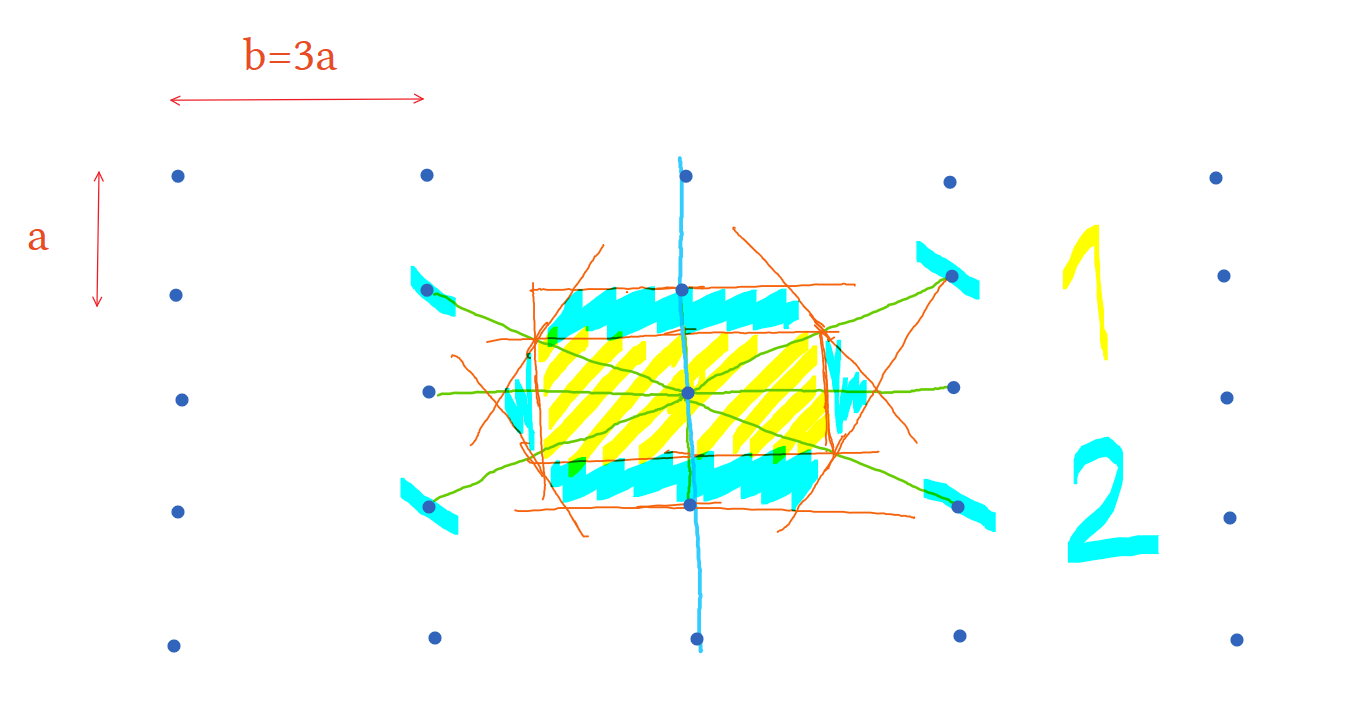
\includegraphics[width = 0.8\linewidth]{Image.png}
    \caption{Primeras dos zonas de Brillouin de una red rectangular.}
    \label{fig:unique}
\end{figure}

Usando el algoritmo geométrico para hallar zonas de Brillouin, se consigue graficar las primeras dos zonas de Brillouin (ver figura \ref{fig:unique}).